\let\bf\bfseries
\let\it\itshape
\section{(7) Транспортные сети. Задача о максимальном потоке. Разрез. Теорема о максимальном потоке и минимальном разрезе. Алгоритм Форда-Фалкерсона (\groth)}
Фактически эта глава~--- просто пересказ параграфов из кормена в правильном порядке. Начнем, с того, что это вообще такое. Итак,
\subsection{Транспортные сети. Задача о максимальном потоке}
\begin{definition}
	{\bfseries Транспортной сетью} называется ориентированный граф $G=\langle V,E\rangle$ с функцией $c\colon V\times V\to\mathbb{N}$, которая называется {\bf\it пропускной способностью}, причем $c(u,v)=0\iff (u,v)\not\in E$, а также двумя выделенными вершинами~--- {\bf\it источником} $s$ и {\bf\it стоком} $t$.
\end{definition}
Внимание! В источник могут входить ребра, а из стока выходить.

Для удобства предполагается, что любая вершина находится на некотором пути от источника к стоку (то есть граф связный).
\begin{example}
	\needpicture
\end{example}
\begin{definition}
	{\bfseries Потоком} называется функция $f\colon V\times V\to\mathbb{R}$, для которой выполняются следующие свойства:
	\begin{enumerate}
		\item $\forall(u,v)\in V\times V\colon f(u,v)\le c(u,v)$
		\item $\forall(u,v)\in V\times V\colon f(u,v)=-f(v,u)$
		\item $\forall u\in V\smallsetminus\{s,t\}\colon \sum_{v\in V} f(u,v)=0$
	\end{enumerate}
	{\bfseries Величиной} потока называется число $|f|\overset{\mathrm{def}}{=}\sum_{v\in V}f(s,v)$.
\end{definition}
Одна из возможных интерпретаций этого~-- электрическая цепь. Тогда все свойства потоков превращаются в правила Кирхгофа.

Обратите внимание, что если есть ребро $(u,v)$ и с потоком $f(u,v)\ne0$, но нет ребра $(v,u)$, то тем не менее $f(v,u)=-f(u,v)\ne0$. Подумайте, почему если между вершинами нет ребра ни в каком направлении, то поток между ними нулевой\footnote{потому что $0=c(u,v)\ge f(u,v)=-f(v,u)\ge -c(v,u)=0$}.
\begin{problem}{\bf (о максимальном потоке)}
	Дана транспортная сеть. Нужно найти в ней поток максимальной величины.
\end{problem}
Базовая идея: взять какой-нибудь (например, тривиальный) поток и увеличивать его, пока можно. Осталось только научиться все это делать, но нужно еще несколько определений.
\begin{definition}
	Для сети $G$ и потока $f$ {\bf\it остаточной пропускной способностью} ребра $(u,v)$ называется величина $c_f(u,v)=c(u,v)-f(u,v)$. {\bf\it Остаточной сетью} $G_f=\langle V,E_f\rangle$ называется сеть на вершинах графа $G$ с множеством ребер $E_f=\{(u,v)\in V\times V|c_f(u,v)>0\}$ с пропускной способностью $c_f$ и теми же источником и стоком.
\end{definition}

Обратите внимание, что если в $G$ есть ребро $(u,v)$, но нет ребра $(v,u)$ (то есть его пропускная способность 0), то остаточная пропускная способность $c_f(v,u)=c(v,u)-f(v,u)=f(u,v)$, то есть если между вершинами есть одно из ребер с ненулевым потоком, то в остаточную сеть попадут оба.
Получается, что $|E_f|\le 2|E|$\label{someshit6}.

\begin{lemma}\label{someshit1} %(о том, как поток в остаточной сети связан с потоком в исходной)
	Пусть $\langle G,c\rangle$~--- транспортная сеть, $f$~--- поток в ней, $G_f$~-- остаточная сеть и в ней задан поток $f'$. Тогда $f+f'$~--- поток в $G$, а его величина $|f+f'|=|f|+|f'|$.
\end{lemma}
\begin{proof}
	Проверим условия на потоки:
	\begin{enumerate}
		\item $$(f+f')(u,v)=f(u,v)+f'(u,v)\le f(u,v)+(c(u,v)-f(u,v))=c(u,v)$$
		\item $$(f+f')(u,v)=f(u,v)+f'(u,v)=-f(v,u)-f'(v,u)=-(f+f')(v,u)$$
		\item $$\sum_{v\in V}(f+f')(u,v)=\sum_{v\in V}f(u,v)+\sum_{v\in V}f'(u,v)=0$$
	\end{enumerate}
	Поэтому это поток.
	
	С величиной все понятно:
	$$|f+f'|=\sum_{v\in V}(f+f')(s,v)=\sum_{v\in V}f(s,v)+\sum_{v\in V}f'(s,v)=|f|+|f'|$$
\end{proof}
\begin{definition}
	{\bf\it Увеличивающим путем} называется простой путь между $s$ и $t$ в $G_f$.
\end{definition}
\begin{lemma}\label{someshit2}
	$G,c,s,t$~--- сеть с потоком $f$, $p$~--- увеличивающий путь в $G_f$. Определим $f_p\colon V\times V\to\mathbb{R}$.
	$$
	f_p(u,v)=
	\begin{cases}
		c_f(p), & (u,v)\in p,\\
		-c_f(p), & (v,u)\in p,\\
		0, & \mathrm{otherwise}
	\end{cases}
	$$
	где $c_f(p)=\min\{c_f(u,v)|(u,v)\in p\}$.
	Тогда $f_p$~--- поток в $G$ с величиной $c_f(p)>0$.
\end{lemma}
\begin{proof}$ $\newline
	\begin{enumerate}
		\item $$f_p(u,v)\le c_f(p)\le c_f(u,v)=c(u,v)-f(u,v)\le c(u,v)$$ если $f(u,v)\ge 0$. Остальные случаи тривиальны.
		\item \ldots
		\item Заметим, что для любой вершины $v$ (не источника и не стока) в путь входит ровно одно ребро $(u,v)$ и ровно одно ребро $(v,w)$, то есть у всех остальных ребер потоки будут нулевые, а у этих они отличаются знаком, поэтому сумма потоков  $\sum_{v\in V}f_p(u,v)=0$.
	\end{enumerate}
\end{proof}
Из лемм~\ref{someshit1} и \ref{someshit2} следует, что поток на каждом ребре пути может быть увеличен на величину $c_f(p)$ (которая называется {\bf\it пропускной способностью пути}), чтобы не нарушить условия на сумму потоков и ограничение пропускной способности.

Теперь осталось научиться определять, чем максимальный поток отличается от немаксимального. Для этого нужно еще несколько определений и важная теорема, а именно
\subsection{Разрез. Теорема о максимальном потоке и минимальном разрезе}
\begin{definition}
	{\bf\it Разрезом} сети $G$ называется разбиение $V=S\sqcup T$, что $s\in S,t\in T$.
	{\bf\it Чистым потоком} потока $f$ через разрез $(S,T)$ называется $f(S,T)\overset{\mathrm{def}}{=}\sum_{x\in S}\sum_{y\in T}f(x,y)$. 
	{\bf\it Пропускной способностью разреза} называется $c(S,T)\overset{\mathrm{def}}{=}\sum_{x\in S}\sum_{y\in T}c(x,y)$.
	{\bf\it Минимальный разрез}~--- это тот, у которого пропускная способность минимальна.
\end{definition}

\begin{lemma}\label{someshit3}
	Чистый поток через любой разрез равен величине потока.
\end{lemma}
\begin{proof}
	Заметим, что $\sum_{x\in S}\sum_{y\in S}f(x,y)=0$.
	\begin{multline*}
	$$
	\sum_{x\in S}\sum_{y\in T}f(x,y)=\sum_{x\in S}\sum_{y\in V}f(x,y)-\sum_{x\in S}\sum_{y\in S}f(x,y)=\\
	\sum_{x\in S}\sum_{y\in V}f(x,y)=\sum_{y\in V}f(s,y)+\sum_{x\in S\smallsetminus \{s\}}\sum_{y\in V}f(x,y)=\sum_{y\in V}f(s,y)=|f|
	$$
	\end{multline*}
\end{proof}
\begin{lemma}\label{someshit4}
	Величина любого потока не превышает пропускную способность любого разреза.
\end{lemma}
\begin{proof}
	$$
	|f|=\sum_{x\in S}\sum_{y\in T}f(x,y)\le\sum_{x\in S}\sum_{y\in T}c(x,y)=c(S,T)
	$$
\end{proof}
\begin{theorem} {\bf (О максимальном потоке и минимальном разрезе)}\label{maxflowmincut}
	$G,c,s,t$~--- транспортная сеть с потоком $f$. Следующие утверждения эквивалентны:
	\begin{enumerate}
		\item $f$~--- максимальный поток в $G$.
		\item Остаточная сеть $G_f$ не содержит увеличивающих путей.
		\item $|f|=c(S,T)$ для некоторого разреза $(S,T)$.
	\end{enumerate}
\end{theorem}
\begin{proof}$ $\newline %dirty hack to newline
	\begin{itemize}
		\item[$\mathrm{1}\Rightarrow\mathrm{2}$] Если есть увеличивающий путь, то по лемме~\ref{someshit2} можно построить поток со строго большей величиной, то есть $f$ не максимальный.
		\item[$\mathrm{2}\Rightarrow\mathrm{3}$] Предположим, что нет увеличивающего пути. Определим $S=\{v\in V|\exists p\colon s\to v\textrm{ in }G_f\}, T=V\smallsetminus S$. Понятно, что это разрез. В нем для любой пары $(u,v)\in S\times T$ выполняется $f(u,v)=c(u,v)$, потому что иначе бы ребро $(u,v)$ попало бы в $E_f$ (напомню, что там находятся только те ребра, у которых положительная остаточная пропускная способность) а значит существовал бы путь из $s$ в $v$, это противоречит $v\in T$. $$|f|=\sum_{x\in S}\sum_{y\in T}f(x,y)=\sum_{x\in S}\sum_{y\in T}c(x,y)$$
		\item[$\mathrm{3}\Rightarrow\mathrm{1}$] Из леммы~\ref{someshit4} следует, что $|f|\le c(S,T)$. Поэтому если достигается равенство, то $f$~--- максимальный.
	\end{itemize}
\end{proof}

Теперь мы умеем все доказывать, чтобы описать алгоритм из базовой идеи, который называется
\subsection{Алгоритм Форда-Фалкерсона}
\begin{algorithm}[H]
\DontPrintSemicolon
\SetKwIF{If}{ElseIf}{Else}{if}{:}{elif}{else}{}
\SetKwFor{For}{for}{:}{}
\SetKwFor{While}{while}{:}{}
\SetKwFor{ForEach}{foreach}{:}{}
\SetKwFunction{FFA}{FFA}
\SetKwProg{Fn}{}{:}{}
\Fn{\FFA{$G=\langle V,E\rangle$,$c$,$s$,$t$}}{
    \ForEach{$(u, v) \in E$}{
        $f(u, v)$ := 0\;
        $f(v, u)$ := 0\;
    }
    \While{$\exists p\colon s\to t,p\subseteq E_f$}{
        $c_f(p)$ := $\min\{c_f(u,v)|(u,v)\in p\}$\;
        \ForEach{$(u, v) \in p$}{
            $f(u,v)$ += $c_f(p)$\;
            $f(v,u)$ := $-f(u,v)$\;
        }
    }
}
\end{algorithm}

На практике, понятно, он возникает в основном только с целыми числами. Проблема этого алгортима в том, что не указано, как именно нужно искать увеличивающий путь. Если искать его неудачно\footnote{а еще если значения пропускных способностей иррациональные, пример можно найти в \href{https://en.wikipedia.org/wiki/Ford-Fulkerson_algorithm}{англоязычной википедии}}, то алгоритм может и зависнуть.

\begin{comment}
\begin{example}
Вот в такой сети алгоритм будет выполняться бесконечно долго и не будет сходиться к правильному ответу:

\tikzset{every picture/.style={line width=0.75pt}} %set default line width to 0.75pt  
\begin{center}      
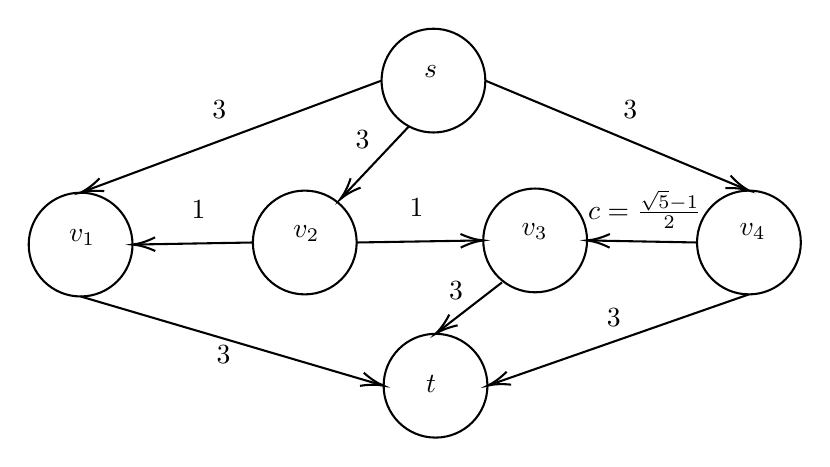
\begin{tikzpicture}[x=0.75pt,y=0.75pt,yscale=-1,xscale=1]
%uncomment if require: \path (0,235); %set diagram left start at 0, and has height of 235
%Shape: Circle [id:dp062013207712154794] 
\draw   (347,37) .. controls (347,23.19) and (358.19,12) .. (372,12) .. controls (385.81,12) and (397,23.19) .. (397,37) .. controls (397,50.81) and (385.81,62) .. (372,62) .. controls (358.19,62) and (347,50.81) .. (347,37) -- cycle ;
%Straight Lines [id:da12150689014580618] 
\draw    (347,37) -- (203.87,90.3) ;
\draw [shift={(202,91)}, rotate = 339.57] [color={rgb, 255:red, 0; green, 0; blue, 0 }  ][line width=0.75]    (10.93,-3.29) .. controls (6.95,-1.4) and (3.31,-0.3) .. (0,0) .. controls (3.31,0.3) and (6.95,1.4) .. (10.93,3.29)   ;
%Shape: Circle [id:dp22596873627634528] 
\draw   (177,116) .. controls (177,102.19) and (188.19,91) .. (202,91) .. controls (215.81,91) and (227,102.19) .. (227,116) .. controls (227,129.81) and (215.81,141) .. (202,141) .. controls (188.19,141) and (177,129.81) .. (177,116) -- cycle ;
%Shape: Circle [id:dp4804239996566908] 
\draw   (499,115) .. controls (499,101.19) and (510.19,90) .. (524,90) .. controls (537.81,90) and (549,101.19) .. (549,115) .. controls (549,128.81) and (537.81,140) .. (524,140) .. controls (510.19,140) and (499,128.81) .. (499,115) -- cycle ;
%Shape: Circle [id:dp2788070487240514] 
\draw   (285,115) .. controls (285,101.19) and (296.19,90) .. (310,90) .. controls (323.81,90) and (335,101.19) .. (335,115) .. controls (335,128.81) and (323.81,140) .. (310,140) .. controls (296.19,140) and (285,128.81) .. (285,115) -- cycle ;
%Shape: Circle [id:dp8904744358830853] 
\draw   (396,114) .. controls (396,100.19) and (407.19,89) .. (421,89) .. controls (434.81,89) and (446,100.19) .. (446,114) .. controls (446,127.81) and (434.81,139) .. (421,139) .. controls (407.19,139) and (396,127.81) .. (396,114) -- cycle ;
%Shape: Circle [id:dp6392423508319897] 
\draw   (348,184) .. controls (348,170.19) and (359.19,159) .. (373,159) .. controls (386.81,159) and (398,170.19) .. (398,184) .. controls (398,197.81) and (386.81,209) .. (373,209) .. controls (359.19,209) and (348,197.81) .. (348,184) -- cycle ;
%Straight Lines [id:da18206882445512274] 
\draw    (360,59.25) -- (328.37,92.79) ;
\draw [shift={(327,94.25)}, rotate = 313.32] [color={rgb, 255:red, 0; green, 0; blue, 0 }  ][line width=0.75]    (10.93,-3.29) .. controls (6.95,-1.4) and (3.31,-0.3) .. (0,0) .. controls (3.31,0.3) and (6.95,1.4) .. (10.93,3.29)   ;
%Straight Lines [id:da4116158387637876] 
\draw    (397,37) -- (522.15,89.23) ;
\draw [shift={(524,90)}, rotate = 202.65] [color={rgb, 255:red, 0; green, 0; blue, 0 }  ][line width=0.75]    (10.93,-3.29) .. controls (6.95,-1.4) and (3.31,-0.3) .. (0,0) .. controls (3.31,0.3) and (6.95,1.4) .. (10.93,3.29)   ;
%Straight Lines [id:da6393442444559655] 
\draw    (285,115) -- (229,115.97) ;
\draw [shift={(227,116)}, rotate = 359.01] [color={rgb, 255:red, 0; green, 0; blue, 0 }  ][line width=0.75]    (10.93,-3.29) .. controls (6.95,-1.4) and (3.31,-0.3) .. (0,0) .. controls (3.31,0.3) and (6.95,1.4) .. (10.93,3.29)   ;
%Straight Lines [id:da9200946912364403] 
\draw    (335,115) -- (394,114.03) ;
\draw [shift={(396,114)}, rotate = 539.06] [color={rgb, 255:red, 0; green, 0; blue, 0 }  ][line width=0.75]    (10.93,-3.29) .. controls (6.95,-1.4) and (3.31,-0.3) .. (0,0) .. controls (3.31,0.3) and (6.95,1.4) .. (10.93,3.29)   ;
%Straight Lines [id:da3038479987969267] 
\draw    (499,115) -- (448,114.04) ;
\draw [shift={(446,114)}, rotate = 361.08000000000004] [color={rgb, 255:red, 0; green, 0; blue, 0 }  ][line width=0.75]    (10.93,-3.29) .. controls (6.95,-1.4) and (3.31,-0.3) .. (0,0) .. controls (3.31,0.3) and (6.95,1.4) .. (10.93,3.29)   ;
%Straight Lines [id:da4917567000192774] 
\draw    (202,141) -- (346.08,183.43) ;
\draw [shift={(348,184)}, rotate = 196.41] [color={rgb, 255:red, 0; green, 0; blue, 0 }  ][line width=0.75]    (10.93,-3.29) .. controls (6.95,-1.4) and (3.31,-0.3) .. (0,0) .. controls (3.31,0.3) and (6.95,1.4) .. (10.93,3.29)   ;
%Straight Lines [id:da16844845591921243] 
\draw    (524,140) -- (399.89,183.34) ;
\draw [shift={(398,184)}, rotate = 340.75] [color={rgb, 255:red, 0; green, 0; blue, 0 }  ][line width=0.75]    (10.93,-3.29) .. controls (6.95,-1.4) and (3.31,-0.3) .. (0,0) .. controls (3.31,0.3) and (6.95,1.4) .. (10.93,3.29)   ;
%Straight Lines [id:da21552238806972335] 
\draw    (405,134.25) -- (374.58,157.78) ;
\draw [shift={(373,159)}, rotate = 322.28] [color={rgb, 255:red, 0; green, 0; blue, 0 }  ][line width=0.75]    (10.93,-3.29) .. controls (6.95,-1.4) and (3.31,-0.3) .. (0,0) .. controls (3.31,0.3) and (6.95,1.4) .. (10.93,3.29)   ;

% Text Node
\draw (195,107.4) node [anchor=north west][inner sep=0.75pt]    {$v_{1}$};
% Text Node
\draw (366,28.4) node [anchor=north west][inner sep=0.75pt]    {$s$};
% Text Node
\draw (367,177.4) node [anchor=north west][inner sep=0.75pt]    {$t$};
% Text Node
\draw (303,105.4) node [anchor=north west][inner sep=0.75pt]    {$v_{2}$};
% Text Node
\draw (413,104.4) node [anchor=north west][inner sep=0.75pt]    {$v_{3}$};
% Text Node
\draw (518,104.4) node [anchor=north west][inner sep=0.75pt]    {$v_{4}$};
% Text Node
\draw (333,59.4) node [anchor=north west][inner sep=0.75pt]    {$3$};
% Text Node
\draw (264,45.4) node [anchor=north west][inner sep=0.75pt]    {$3$};
% Text Node
\draw (462,45.4) node [anchor=north west][inner sep=0.75pt]    {$3$};
% Text Node
\draw (254,93.4) node [anchor=north west][inner sep=0.75pt]    {$1$};
% Text Node
\draw (359,92.4) node [anchor=north west][inner sep=0.75pt]    {$1$};
% Text Node
\draw (454,145.4) node [anchor=north west][inner sep=0.75pt]    {$3$};
% Text Node
\draw (378,132.4) node [anchor=north west][inner sep=0.75pt]    {$3$};
% Text Node
\draw (266,163.4) node [anchor=north west][inner sep=0.75pt]    {$3$};
% Text Node
\draw (445,88.4) node [anchor=north west][inner sep=0.75pt]    {$c=\frac{\sqrt{5} -1}{2}$};
\end{tikzpicture}
\end{center}

Величина максимального потока в этой сети равна $7=2\cdot3+1$ (на ребрах $s\to v_1\to t$ и $s\to v_4\to t$ его значение 3, на ребрах $s\to v_2\to v_3\to t$ его значение 1). 
\end{example}
\end{comment}

В предположении, что числа рациональные (их можно свести к целым) и при использовании поиска в глубину или поиска в ширину для нахождения увеличивающего, время его работы составляет $O(|E||f^*|)$, где $f^*$~--- максимальный поток (в случае использования поиска в ширину этот алгоритм называется {\bf\it алгоритмом Эдмондса-Карпа}, для него в секции~\ref{edmonds_karp} мы докажем более точную оценку).

Проанализируем время работы. Первый цикл выполняется за время $\Theta(|E|)$, второй цикл выполняется не более $|f^*|$ раз (потому что величина потока в каждую итерацию увеличивается хотя бы на 1).

Время работы поиска $O(|V|+|E|)=O(|E|)$ (так как наш граф связный, а в нем $|E|\ge |V|-1$, поэтому весь цикл выполняется за время $O(|E||f^*|)$.

\begin{example}
	Алгоритм работает плохо, если найдется неудачный увеличивающий путь:
	\begin{center}
	\tikzset{every picture/.style={line width=0.75pt}} %set default line width to 0.75pt        	
	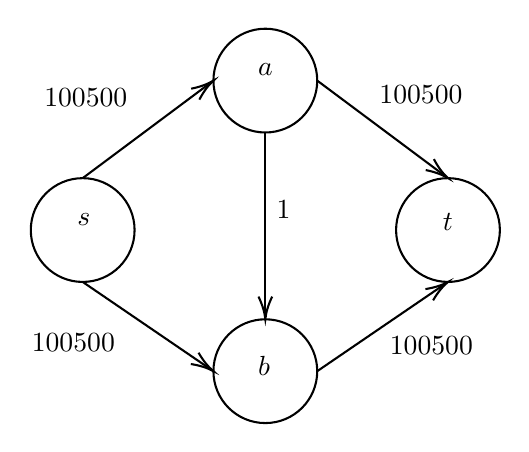
\begin{tikzpicture}[x=0.75pt,y=0.75pt,yscale=-1,xscale=1]
	%uncomment if require: \path (0,235); %set diagram left start at 0, and has height of 235
	%Shape: Circle [id:dp9082962256087861] 
	\draw   (361,99) .. controls (361,85.19) and (372.19,74) .. (386,74) .. controls (399.81,74) and (411,85.19) .. (411,99) .. controls (411,112.81) and (399.81,124) .. (386,124) .. controls (372.19,124) and (361,112.81) .. (361,99) -- cycle ;
	%Shape: Circle [id:dp5154952916611416] 
	\draw   (185,99) .. controls (185,85.19) and (196.19,74) .. (210,74) .. controls (223.81,74) and (235,85.19) .. (235,99) .. controls (235,112.81) and (223.81,124) .. (210,124) .. controls (196.19,124) and (185,112.81) .. (185,99) -- cycle ;
	%Shape: Circle [id:dp11995847002011883] 
	\draw   (273,167) .. controls (273,153.19) and (284.19,142) .. (298,142) .. controls (311.81,142) and (323,153.19) .. (323,167) .. controls (323,180.81) and (311.81,192) .. (298,192) .. controls (284.19,192) and (273,180.81) .. (273,167) -- cycle ;
	%Shape: Circle [id:dp23613876173352422] 
	\draw   (273,27) .. controls (273,13.19) and (284.19,2) .. (298,2) .. controls (311.81,2) and (323,13.19) .. (323,27) .. controls (323,40.81) and (311.81,52) .. (298,52) .. controls (284.19,52) and (273,40.81) .. (273,27) -- cycle ;
	%Straight Lines [id:da26355802505230386] 
	\draw    (210,124) -- (271.35,165.87) ;
	\draw [shift={(273,167)}, rotate = 214.32] [color={rgb, 255:red, 0; green, 0; blue, 0 }  ][line width=0.75]    (10.93,-3.29) .. controls (6.95,-1.4) and (3.31,-0.3) .. (0,0) .. controls (3.31,0.3) and (6.95,1.4) .. (10.93,3.29)   ;
	%Straight Lines [id:da4817769355441677] 
	\draw    (210,74) -- (271.4,28.2) ;
	\draw [shift={(273,27)}, rotate = 503.28] [color={rgb, 255:red, 0; green, 0; blue, 0 }  ][line width=0.75]    (10.93,-3.29) .. controls (6.95,-1.4) and (3.31,-0.3) .. (0,0) .. controls (3.31,0.3) and (6.95,1.4) .. (10.93,3.29)   ;
	%Straight Lines [id:da5670405427917837] 
	\draw    (298,52) -- (298,140) ;
	\draw [shift={(298,142)}, rotate = 270] [color={rgb, 255:red, 0; green, 0; blue, 0 }  ][line width=0.75]    (10.93,-3.29) .. controls (6.95,-1.4) and (3.31,-0.3) .. (0,0) .. controls (3.31,0.3) and (6.95,1.4) .. (10.93,3.29)   ;
	%Straight Lines [id:da8857855961648333] 
	\draw    (323,27) -- (384.4,72.8) ;
	\draw [shift={(386,74)}, rotate = 216.72] [color={rgb, 255:red, 0; green, 0; blue, 0 }  ][line width=0.75]    (10.93,-3.29) .. controls (6.95,-1.4) and (3.31,-0.3) .. (0,0) .. controls (3.31,0.3) and (6.95,1.4) .. (10.93,3.29)   ;
	%Straight Lines [id:da2047755307262834] 
	\draw    (323,167) -- (384.35,125.13) ;
	\draw [shift={(386,124)}, rotate = 505.68] [color={rgb, 255:red, 0; green, 0; blue, 0 }  ][line width=0.75]    (10.93,-3.29) .. controls (6.95,-1.4) and (3.31,-0.3) .. (0,0) .. controls (3.31,0.3) and (6.95,1.4) .. (10.93,3.29)   ;
	
	% Text Node
	\draw (206,89.4) node [anchor=north west][inner sep=0.75pt]    {$s$};
	% Text Node
	\draw (382,89.4) node [anchor=north west][inner sep=0.75pt]    {$t$};
	% Text Node
	\draw (293,17.4) node [anchor=north west][inner sep=0.75pt]    {$a$};
	% Text Node
	\draw (293,158.4) node [anchor=north west][inner sep=0.75pt]    {$b$};
	% Text Node
	\draw (302,83.4) node [anchor=north west][inner sep=0.75pt]    {$1$};
	% Text Node
	\draw (190,29.4) node [anchor=north west][inner sep=0.75pt]    {$100500$};
	% Text Node
	\draw (184,147.4) node [anchor=north west][inner sep=0.75pt]    {$100500$};
	% Text Node
	\draw (356.5,148.9) node [anchor=north west][inner sep=0.75pt]    {$100500$};
	% Text Node
	\draw (351.5,27.9) node [anchor=north west][inner sep=0.75pt]    {$100500$};	
	\end{tikzpicture}
	\end{center}
	Поиском в глубину находится путь $s\to a\to b\to t$, поэтому за одну итерацию поток увеличивается всего лишь на единицу.
	
	В следующей итерации может найтись путь $s\to b\to a\to t$ (так как остаточная пропускная способность $b\to a$ теперь $0-(-1)=1$) и он опять уменьшится всего лишь на 1, поэтому нужный поток найдется за 100500 итераций.
\end{example}

\subsection{Применение к паросочетаниям}
Этим алгоритмом можно пользоваться, чтобы найти в двудольном графе $G=\langle V,E\rangle$ максимальное паросочетание. Для этого нам нужно теперь построить транспортную сеть и научиться сопоставлять потокам паросочетания.

Напомню, что мощностью паросочетания называется количество ребер в нем.

Дан двудольный граф $G=\langle V=L\sqcup R,E\rangle$, $L,R$~--- доли. Добавим еще две выделенные вершины $s,t$ (источник и приемник) и построим сеть $G'=\langle V'=V\cup\{s,t\},E'\rangle$, где $E'=\{(s,u)|u\in L\}\cup\{(u,v)|(u,v)\in E\}\cup\{(v,t)|v\in R\}$. У каждого ребра единичная пропускная способность.

\begin{definition}
	Поток называется {\it\bf целочисленным}, если $\forall (u,v)\in V\times V\colon f(u,v)\in\mathbb{Z}$.
\end{definition}
\begin{lemma}
	Каждому паросочетанию в $G$ взаимно однозначно соответствует целочисленный поток $f$ в $G'$ мощности $|f|=|M|$.
\end{lemma}
\begin{proof}
	Для начала построим поток по паросочетанию: если $(u,v)\in M$, то $f(s,u)=f(u,v)=f(v,t)=1$, $f(t,v)=f(v,u)=f(v,s)=-1$, для всех остальных $(u,v)$ $f(u,v)=0$. Понятно, что это поток, и так как чистый поток через разрез $(L\cup\{s\},R\cup\{t\})$ равен $M$, то и величина всего потока равна $|M|$.
	
	Пусть теперь $f$~-- поток в $G'$. Определим $$M=\{(u,v)|u\in L, v\in R, f(u,v)>0\}$$
	
	Поскольку пропускная способность каждого ребра равна 1, в вершину $u\in L$ входит не больше одной единицы потока. Так как она обязана куда-то выходить и поток целочисленный, она выходит по одному ребру. Так что единица положительного потока входит в $u$, согда существует единственная вершина $v\in R$, в которую эта единица входит. То же самое можно сказать про любую вершину $v\in R$, поэтому это паросочетание. Понятно, что величина этого потока равна $|M|$: по построению нашей сети $f(s,v)=0 \forall v\in R\cup\{s,t\}$, поэтому $$|f|=\sum_{v\in V'\smallsetminus\{s\}}f(s,v)=\sum_{v\in L}f(s,v)=|M|$$
\end{proof}

Понятно, что максимальному паросочетанию $M$ соотвествтует максимальный поток (поскольку иначе существует паросочетание $M'$, для которого $|M'|=|f'|>|f|=|M|$).

Чтобы применять условия этой леммы, нужно убедиться, что 
\begin{lemma}
	Алгоритм Форда-Фалкерсона в сети с целочисленной пропускной способностью действительно строит целочисленный поток.
\end{lemma}
\begin{proof}
	Индукция по количеству итераций цикла.
\end{proof}
